\documentclass[12pt, a4paper]{article}
\usepackage[a4paper, includeheadfoot, mag=1000, left=2cm, right=1.5cm, top=1.5cm, bottom=1.5cm, headsep=0.8cm, footskip=0.8cm]{geometry}
% Fonts
\usepackage{fontspec, unicode-math}
\setmainfont[Ligatures=TeX]{PT Serif}
\setmonofont{CMU Typewriter Text}
\usepackage[english, russian]{babel}
% Indent first paragraph
\usepackage{indentfirst}
\setlength{\parskip}{5pt}
% Diagrams
\usepackage{graphicx}
\usepackage{float}
% Page headings
\usepackage{fancyhdr}
\pagestyle{fancy}
\renewcommand{\headrulewidth}{0pt}
\setlength{\headheight}{16pt}
% new font       name                fontname in system
% \newfontfamily\namefont[Scale=1.2]{Gloria Hallelujah}
\fancyhead{}
% Use case template
\usepackage{xifthen}
\newcommand{\uctitle}[1]{\renewcommand{\givenuctitle}{#1}}
\newcommand{\givenuctitle}{Не указано}
\newcommand{\ucgoal}[1]{\renewcommand{\givenucgoal}{#1}}
\newcommand{\givenucgoal}{Не указано}
\newcommand{\ucscenario}[1]{\renewcommand{\givenucscenario}{#1}}
\newcommand{\givenucscenario}{}
\newcommand{\ucextensions}[1]{\renewcommand{\givenucextensions}{#1}}
\newcommand{\givenucextensions}{}
\newenvironment{usecase}{}{
  \noindent\fbox{
    \parbox{0.98\textwidth}{
      \vspace{2mm}
      \textbf{\large \givenuctitle}\\[3mm]
      \textbf{Цель:} \givenucgoal\\[2mm]
      \textbf{Сценарий:}
      \begin{enumerate}\givenucscenario\end{enumerate}
      \textbf{Расширения:}
      \begin{itemize}\givenucextensions\end{itemize}
    }
  }
}
\newenvironment{usecasenoext}{}{
  \noindent\fbox{
    \parbox{0.98\textwidth}{
      \vspace{2mm}
      \textbf{\large \givenuctitle}\\[3mm]
      \textbf{Цель:} \givenucgoal\\[2mm]
      \textbf{Сценарий:}
      \begin{enumerate}\givenucscenario\end{enumerate}
    }
  }
}

\begin{document}

% Title page
\begin{titlepage}
\begin{center}

\textsc{«УНИВЕРСИТЕТ ИТМО»\\[4mm]
Кафедра вычислительной техники}
\vfill
\textbf{КУРСОВАЯ РАБОТА}\\[4mm]
по дисциплине:\\[2mm]
\textbf{Программирование интернет-приложений}\\[16mm]
\end{center}

\begin{flushright}
Выполнили: \\[4mm]
Калугина Марина Максимовна \\[2mm]
Каюков Иван Алексеевич \\[2mm]
Группа P3202
\end{flushright}

\begin{center}
\vfill
Санкт-Петербург\\[2mm]
2018 г.

\end{center}
\end{titlepage}



\begin{center}
\textsc{Darknet RoboGit \&\& RoboStore}
\vspace{12mm}
\end{center}
\tableofcontents
\newpage

% Contents

\section{О проекте}

Предметом разработки является RoboGit -- платформа для хостинга робототехнических проектов,
который основан на системе контроля версий Git с поддержкой markdown и
RoboStore -- интернет-магазин с товарами для робототехники на домене .onion,
поддерживающий оплату криптовалютой.
Платформа позволяет пользователям формировать заказ на покупку необходимого для
текущего проекта комплекта деталий и совершать покупку необходимого в один клик.

\subsection{Цель создания}

\begin{itemize}
  \item{Предоставляние пользователям возможности размещения робототехнических
    проектов и организации пользовательских проектов
    с помощью системы контроля версий Git.}
  \item{Поддержание анонимности пользователей.}
  \item{Организация интернет-магазина с товарами для робототехники.}
  \item{Предоставляние пользователям возможности упрощенно совершать покупку
    необходимых для проекта товаров.}
\end {itemize}

\subsection{Целевая аудитория}

Плохие парни.

\subsection{Описание прецедентов}

\begin{usecase}
\uctitle{Регистрация и авторизация}
\ucgoal{Завести аккаунт в cистеме, создать персонажа}
\ucscenario{
  \item Незарегистрированный/неавторизироанный пользователь имеет доступ ко всем 
    страницам платформы, кроме своего профиля и создания нового репозитория.
  \item При попытке перейти к себе в профиль (главную сстраницу RoboGit) или при
    попытке создания нового репозитория открывается форма авторизации
    с ссылкой на форму регистрации.
  \item Пользователь автооризируется или переходит на страницу регистрации,
    заполняет поля и отправляет форму.
  \item Система перенаправляет на страницу личного профиля пользователя.
}
\ucextensions{
  \item Ошибка при авторизации (неверный логин/пароль) или ошибка при регистрации
    (адрес электронной почты уже используется, пароль слишком короткий)
    предотвращает переход на страницу личного профиля.
}
\end{usecase}

\begin{usecase}
\uctitle{Создание нового репозитория}
\ucgoal{Создать новый репозиторий}
\ucscenario{
  \item Авторизированный пользователь переходит на страницу содания нового репозитория.
  \item Открывается форма для ввода имени репозитория и его описания.
  \item После успешной отправки формы появляется страница, в которой описывается
    как создать репозиторий с командной строки или импортировать код.
}
\ucextensions{
  \item Ошибка при создании репозитория (репозиторий уже с таким именем уже
    существует в данном аккаунте) предотвращает создание репозитория.
}
\end{usecase}

\begin{usecasenoext}
\uctitle{Работа с существующим репозиторием}
\ucgoal{Держить актуальные версии проектов в RoboGit-e}
\ucscenario{
  \item Работа с существующим репозиторием ведется через командную строку
    пользоваткльсткого персонатьлного компьютера.
}
\end{usecasenoext}

\begin{usecase}
\uctitle{Просмотр пользовательских репозиториев}
\ucgoal{Просмотр пользователями репозиториев других пользователей,
  знакомство с кодом и описаниями.}
\ucscenario{
  \item Пользователь открывает страницу репозитория.
  \item Платформа предоставляет обзор всех файлов, находящихся в репозитории.
  \item Файлы, написанные при помощи языка разметки Markdown и имеющие
    расширение .md, представляются на платформе в виде страницы-публикации.
}
\ucextensions{
  \item В файлах с расширением .md можно указывать товары из RoboStore
    для добавления из в корзины пользователей.
}
\end{usecase}

\begin{usecase}
\uctitle{Оценка пользовательских репозиториев}
\ucgoal{Поощрение интересных проектов, создание топа лучших проектов RoboGit.}
\ucscenario{
  \item Пользователь отмечает понравившиеся репозитории, нажимая
    кнопку stars на странице репозитория.
  \item Система сохраняет информацию о количестве stars
    для текущего репозитория.
}
\ucextensions{
  \item Stars влияют на положении репозитория в топе.
  \item В пользовательских профилях для каждого репозитория
    отображается количество stars.
}
\end{usecase}

\begin{usecasenoext}
\uctitle{Формирование заказа на покупку из пользовательских проектов}
\ucgoal{Добавление товара из проекта в корзину в один клик для дальнейшей покупки.}
\ucscenario{
  \item Пользователь открывает файл с расширением .md, в котором есть товар из RoboStore.
  \item При нажатии на наименование товара, он отправляется в пользовательскую корзину.
}
\end{usecasenoext}

\begin{usecasenoext}
\uctitle{Просмотр профиля пользователей}
\ucgoal{Просмотр пользовательских профилей, знакомство с репозиториями пользователя.}
\ucscenario{
  \item Пользователь открывает страницу пользовательского профиля.
  \item Платформа предоставляет обзор всех репозиториев пользователя.
}
\end{usecasenoext}

\begin{usecasenoext}
\uctitle{Просмотр главной страницы магазина}
\ucgoal{Ознакомить пользователей с асортиментом магазина.}
\ucscenario{
  \item Главная страница платформы содержит краткое описание товара.
  \item Пользователь имеет возможность выбрать категорию товара, при выборе
    катогроии на странице остаются товары только выбранной категории.
  \item Платформа позволяет отфильтровать товары. Фильтры для каждой
    категории товаров индивидуальны.
}
\end{usecasenoext}

\begin{usecasenoext}
\uctitle{Просмотр страницы товара}
\ucgoal{Позволяет пользователем подробнее ознакомиться с товаром.}
\ucscenario{
  \item С краткого описания товара на главной стронице RoboStore пользователь
    может перейти к просмотру страницы товара, нажав на кнопку "Подробнее".
  \item После нажатия кнопки пользователь переходит на страницу с подробным
    описанием товара (характеристики, описание).
}
\end{usecasenoext}

\begin{usecasenoext}
\uctitle{Выбор фильтров для товаров}
\ucgoal{Позволить пользователям фильтровать товар по характеристикам,
  зависящим от категории товара.}
\ucscenario{
  \item После выбора категории товаров, пользователю становится доступен 
    выбор категорий для фильтров товаров.
  \item Пользователь может установить необходмые ему фильтры и отправить форму.
  \item После отправки формы платформа оставит товары, удовлетворяющие фильтру.
}
\end{usecasenoext}

\begin{usecasenoext}
\uctitle{Добавление товаров в корзину}
\ucgoal{Формирование пользовательской корзины для дальнейшего оформления заказа.}
\ucscenario{
  \item С краткого описания товара на главной стронице RoboStore пользователь может
    перейти к просмотру страницы товара, нажав на кнопку "В корзину".
  \item После этого платформа отправляет товар ы пользовательскую корзину.
}
\end{usecasenoext}

\begin{usecase}
\uctitle{Просмотр корзины}
\ucgoal{Ознакомить пользователя с корзиной для дальнейшего формирования заказа.}
\ucscenario{
  \item Пользователь открывает страницу с личной корзиной.
  \item В один клик пользователь может изменить количество товаров в заказе,
    удалить товар из корзины или начать оформлять заказ.
}
\ucextensions{
  \item Если корзина пуста, платформа предлагает перейти на главную страницу RoboStore.
}
\end{usecase}

\begin{usecasenoext}
\uctitle{Формирование заказа}
\ucgoal{Сформировать заказ для покупки товара.}
\ucscenario{
  \item Пользователь нажимает кнопку формирования товара.
  \item Открывается страница, которая предоставляет пользователю ссылку для
    связи с телеграм-ботом для дальнейшего формирования заказа.
}
\end{usecasenoext}

\subsection{UML-диаграмма прецедентов}

\begin{figure}[H]
  \centering
  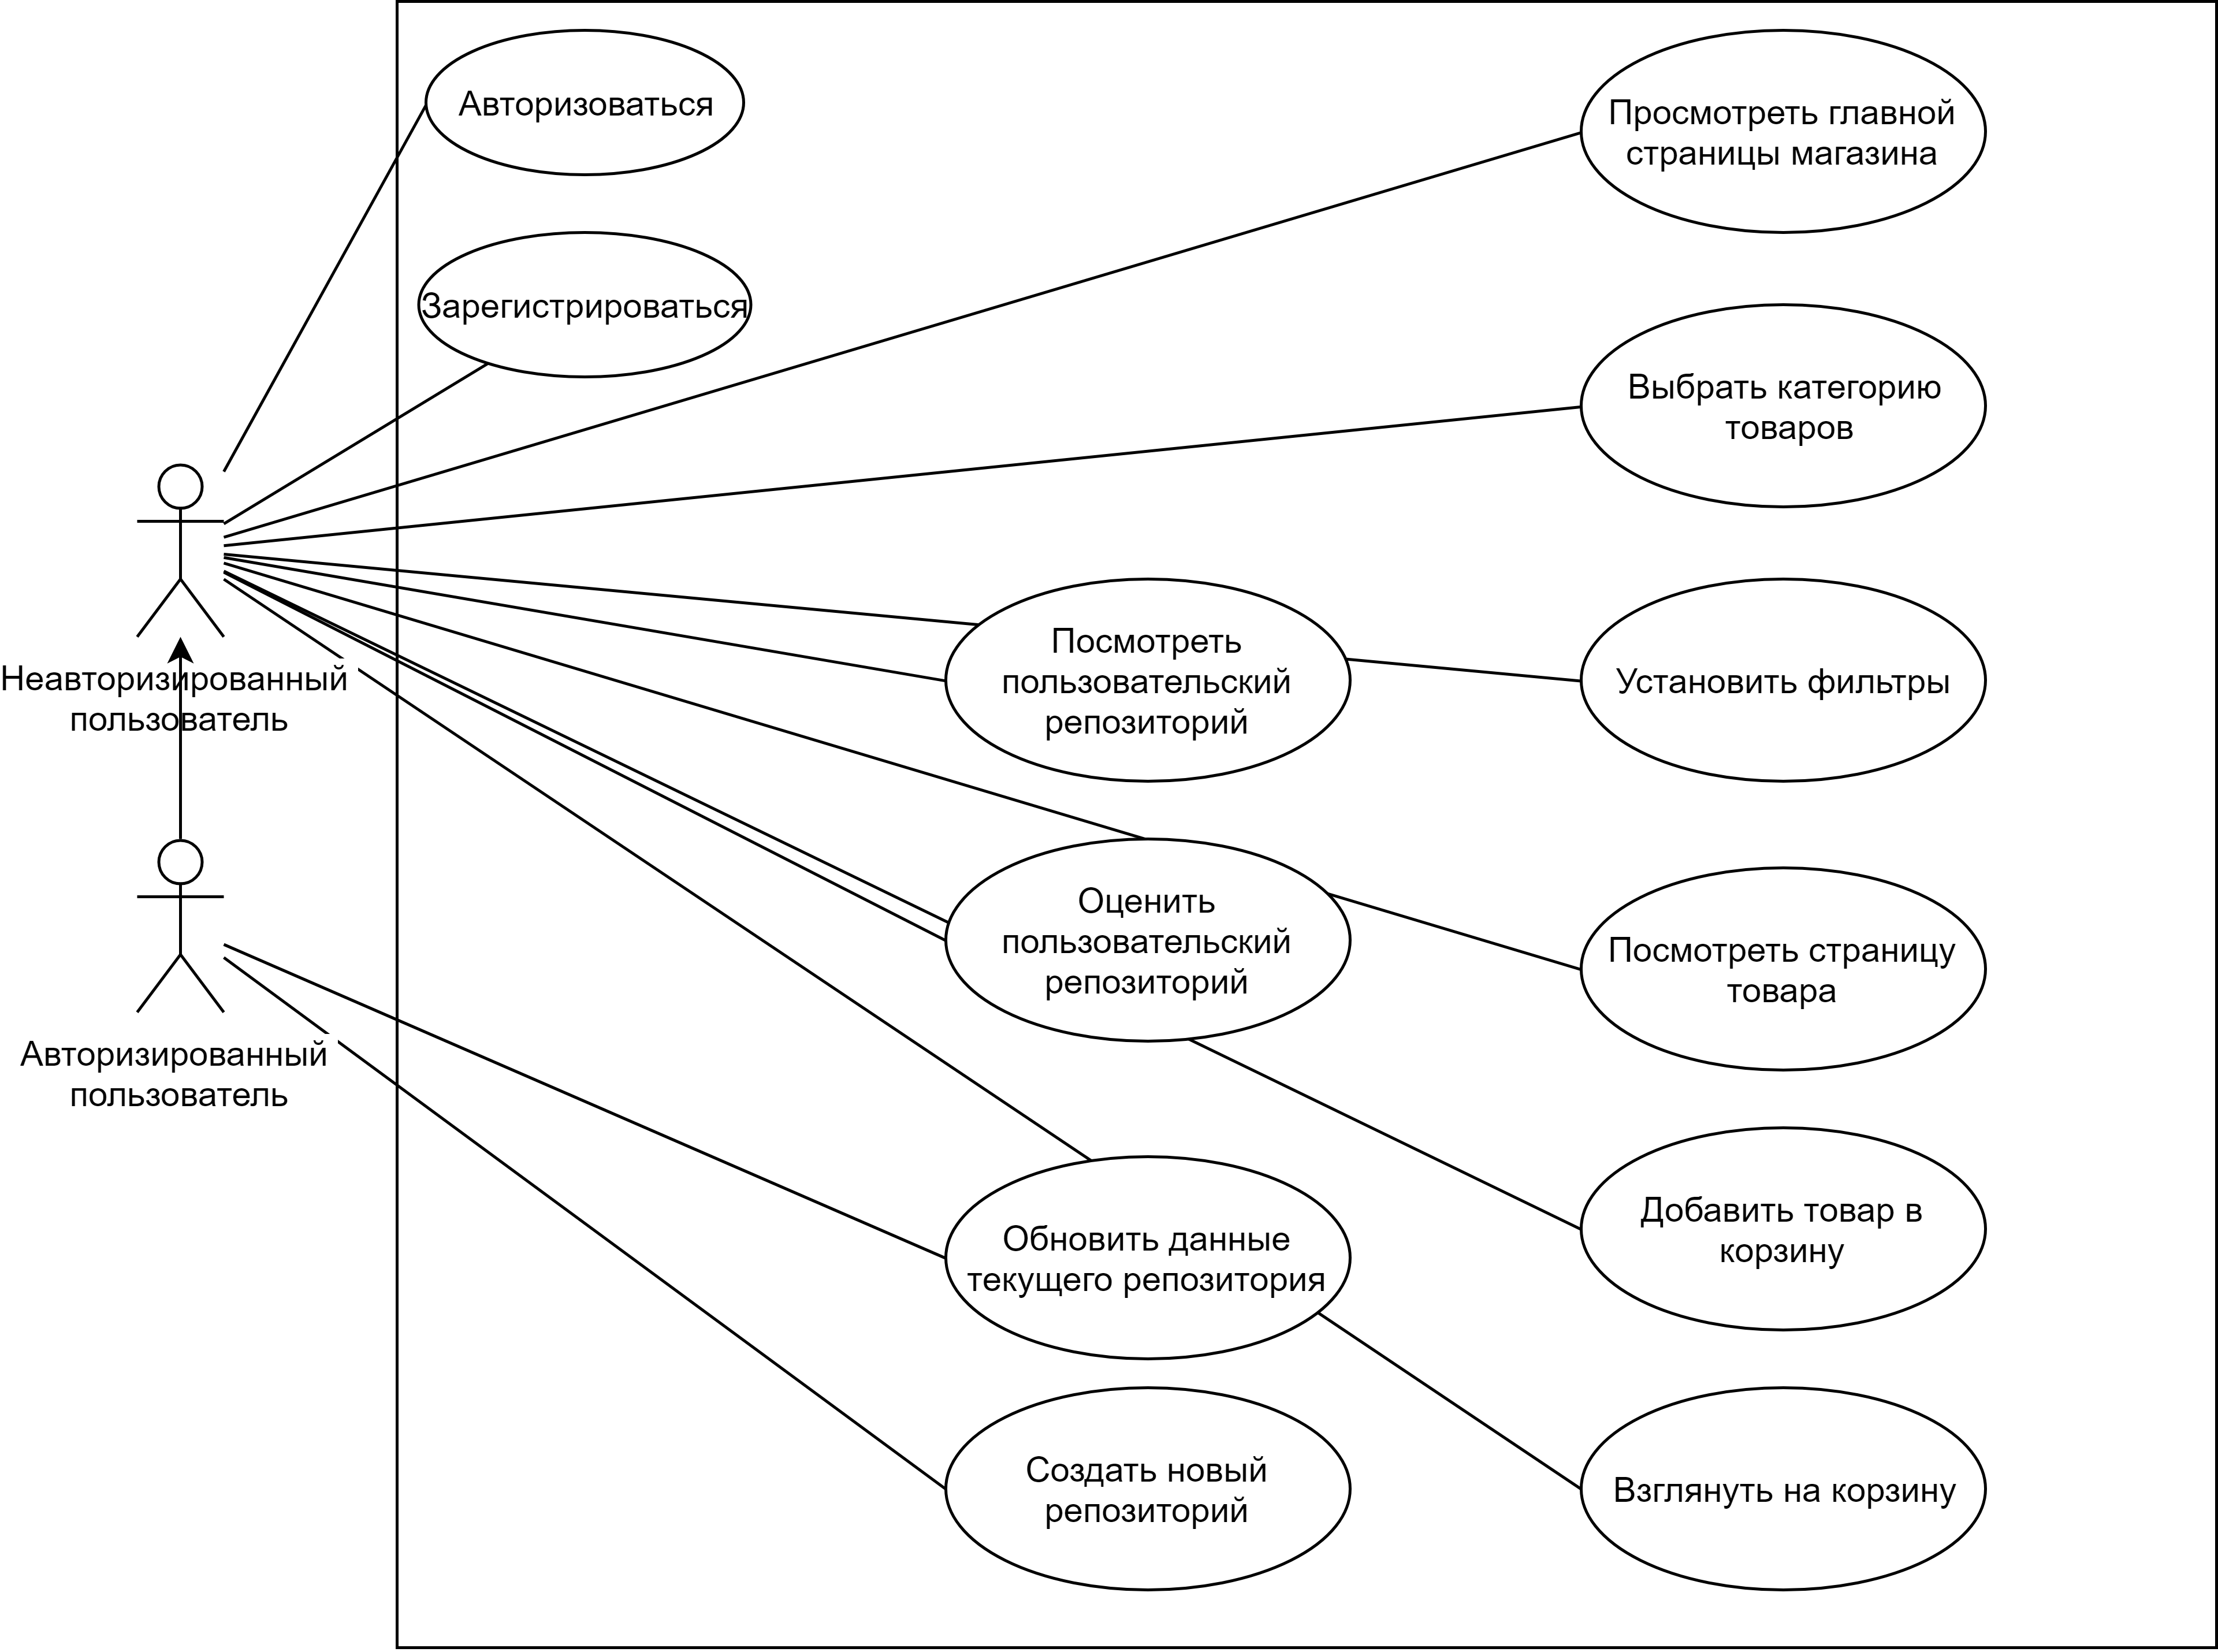
\includegraphics[width=16cm]{uml-precedents.png}
  \caption{UML-диаграмма прецедентов}
\end{figure}

\section{Требования к аппаратно-программному обеспечению}

\subsection{Требования к серверному обеспечению}

Система, которая обеспечивает выполнение программных продуктов сервера 
приложений и хранение данных платформы, должна отвечать следующим требованиям:

\begin{enumerate}
\item Наличие операционной системы Linux
\item Наличие сервера ба данных PostgreSQL версии 9.6 или выше
\item Наличие сервера приложений GlassFish версии 4.1.2 или выше
\item Наличие на сервере JDK 8
\end{enumerate}

\subsection{Требования к клиентскому обеспечению}

Браузерный интерфейс разрабатывается с учетом следующих требований к
программному обеспечению на стороне пользователя:

\begin{enumerate}
\item Веб-браузер Tor версии 8.01 или выше
\item Включенный интерпретатор сценариев JavaScript.
\item Отсутствие запрета веб-страницам платформы доступа к внешним ресурсам,
  а именно изображениям, шрифтам, таблицам стилей CSS и сценариям JavaScript,
  в том числе блокировщиками рекламы.
\end{enumerate}

\section{Требования к архитектуре системы}

\subsection{Уровень back-end}

\begin{enumerate}
\item Уровень back-end основывается на \textit{Spring} версии 5 или выше.
\item Взаимодействие между уровнями back-end и front-end организуется
  посредством REST API.
\item Для доступа к БД использeтся \textit{Spring Data.}
\item Серверное приложение должно отправлять пользователям еженедельное 
  новостноe сообщение электронной почты, используя \textit{JavaMail API}.
\item Серверное приложение должно логировать все вызовы методов на уровне 
  бизнес-логики системы с использованием технологии \textit{Spring AOP}
  и \textit{AspectJ}.
\item Ролевое разграничение доступа к внутренним разделам системы 
  организовано с помощью технологии \textit{Spring Security}.
\item Доступ пользователей в систему осуществляется через систему 
  "единого входа" (Single Sign On). В качестве провайдера SSO использована 
  система \textit{ForgeRock OpenAM}, развёрнутая на отдельном экземпляре 
  (домене) сервера приложений.
\end{enumerate}

\subsection{Уровень front-end}

\begin{enumerate}
\item Уровень front-end строится на \textit{ReactJS + Redux} 
  с использованием ES6 и JSX и набора
  компонентов \textit{Belle}.
\item Веб-интерфейс адаптирован для отображения в трех режимах:
  \begin{itemize}
  \item \textit{Десктопном}: ширина экрана больше 1105px
  \item \textit{Планшетном}: ширина экрана больше 687px и меньше 1105px
  \item \textit{Мобильном}: ширина экрана меньше 687px
  \end{itemize}
\end{enumerate}

\subsection{Telegram-бот}
\label{telegram-bot}

Для сохранения анонимности пользователей оформление заказа происходит
через телеграм-бота.

\begin{enumerate}
\item Telegram-бот отправляет инструкции и ссылку для оплаты заказа.
\item Telegram-бот позволяет определить время и место доставки заказа.
\end{enumerate}

\section{Требования к надежности и безопасности системы}

\begin{enumerate}
\item Серверное приложение должно содержать механизмы защиты от
  уязвимостей, входящих в список OWASP TOP-10.
\item Пароли пользователей должны содержать не менее восьми 
  символов и храниться как криптографический хэш.
\end{enumerate}

\section{Архитектура системы}

\begin{figure}[H]
  \centering
  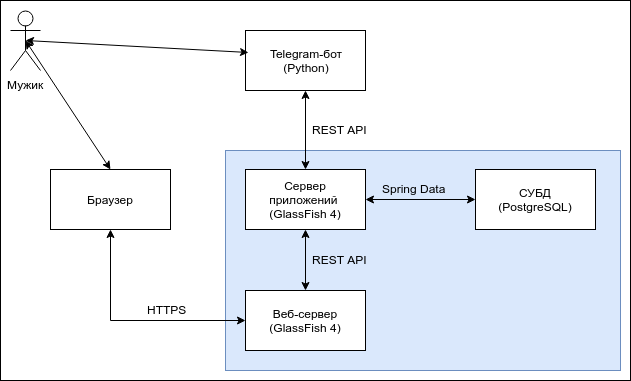
\includegraphics[width=16cm]{system-arch.png}
  \caption{Архитектура системы}
\end{figure}

\section{Прототипы интерфейсов}

% Just an example, how to include pictures:
% \begin{figure}[H]
%  \centering
%  \includegraphics[width=23cm]{ui-mockup-mobile.png}
%  \caption{Мобильные интерфейсы}
%\end{figure}

\end{document}
